\chapter{The software process}
The \emph{software process} is not new. It is just a matter of applying engineering approach to software production.

The main difference with respect to tradition engineering is that software engineering is only 50 years old and it has limited theories and laws. Those issues affect the maturity of customers and managers which, nowadays, is very variable.

\section{Activities}
Goal is to produce software, including documents, data and code, with defined, predictable process properties (cost, duration, \dots) and product properties which defines product quality (functionality, reliability, \dots).
\begin{enumerate}
\item Requirements: what the software should do;
\item Design: definition and organization of physical (files and directories) and logical (functions, classes, packages, subsystems) units;
\item Implementation: source code writing (and generation of executable code) and units integration.
\end{enumerate}
Logically, each activity depends on the previous one. Those dependencies make software not soft.

First approach is to do these activities in sequence. In practice, feedbacks and recycles must be provided. At the end of each activity, a document (or source code) is produced.

\paragraph{The V \& V activities}
The software process may have a lot of defects. The idea is to find and fix them as soon as they are discovered. \emph{Verification and validation} activities control the correctness of:
\begin{itemize}
\item the requirements: customer needs are known and understood and the requirements document is consistent;
\item the design: it is capable of supporting the requirements and it is consistent;
\item the code: it is capable of supporting the requirements and the design and it is consistent (syntactic checks).
\end{itemize}

\paragraph{The management activities}
\begin{itemize}
\item Project management
\begin{itemize}
\item Assigns work and monitors progress;
\item Estimates and control budget.
\end{itemize}
\item Configuration management
\begin{itemize}
\item Identifies and stores documents and units;
\item Keeps track of relationships and history (version control).
\end{itemize}
\item Quality assurance
\begin{itemize}
\item Defines quality goals;
\item Defines how work will be done;
\item Controls results;
\item May repeat some V \& V activities.
\end{itemize}
\end{itemize}

\begin{figure}[hbtp]
\centering
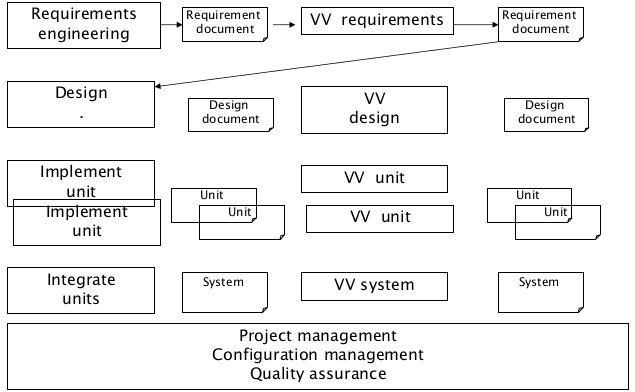
\includegraphics[scale=0.5]{images/software_activities.png}
\caption{Production + VV activities}
\end{figure}

\section{Phases}
Development is only the first part of the game. 

\begin{figure}[hbtp]
\centering
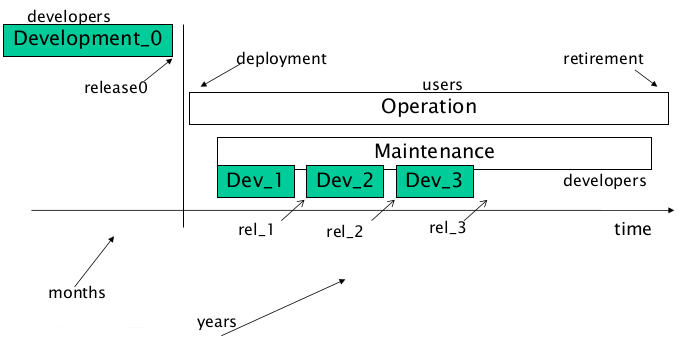
\includegraphics[scale=0.4]{images/software_phases.jpg}
\caption{Software phases}
\end{figure}

\paragraph{Operation}
\emph{Operation} is made by the users until retirement. Companies try to keep software as long as possible, i.e.\@ tens of years. A software used for a short amount of time, is not a good one. 

\paragraph{Maintenance}
\emph{Maintenance} can be seen as a sequence of developments. It starts immediately after the first release and lasts until retirement.

First development is usually longer, next developments are constrained by previous ones and related choices. After years, the constraints are so many that changes become impossible.

\begin{figure}[hbtp]
\centering
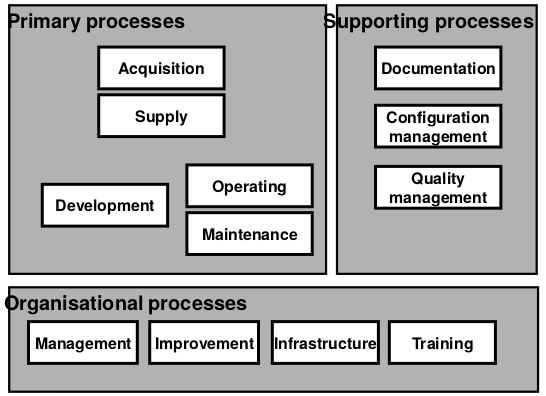
\includegraphics[scale=0.4]{images/iso_iec_12207.png}
\caption{ISO/IEC 12207}
\end{figure}

\section{The system process}
\emph{Embedded software} requires system process:

\begin{enumerate}
\item System requirements;
\item System design;
\item software development (requirements, design, implementation, test and integration);
\item System integration and test.
\end{enumerate}

\begin{figure}[hbtp]
\centering
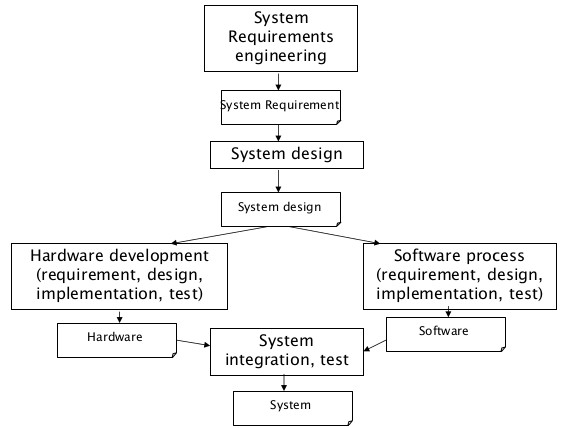
\includegraphics[scale=0.4]{images/system_process.jpg}
\caption{The system process}
\end{figure}